\section{Performance Evaluation and Analysis}
\label{sec:evaluation}

\subsection{DEPOT Performance}
\label{sec:o3_real}

\begin{figure}[t]
  \centering
  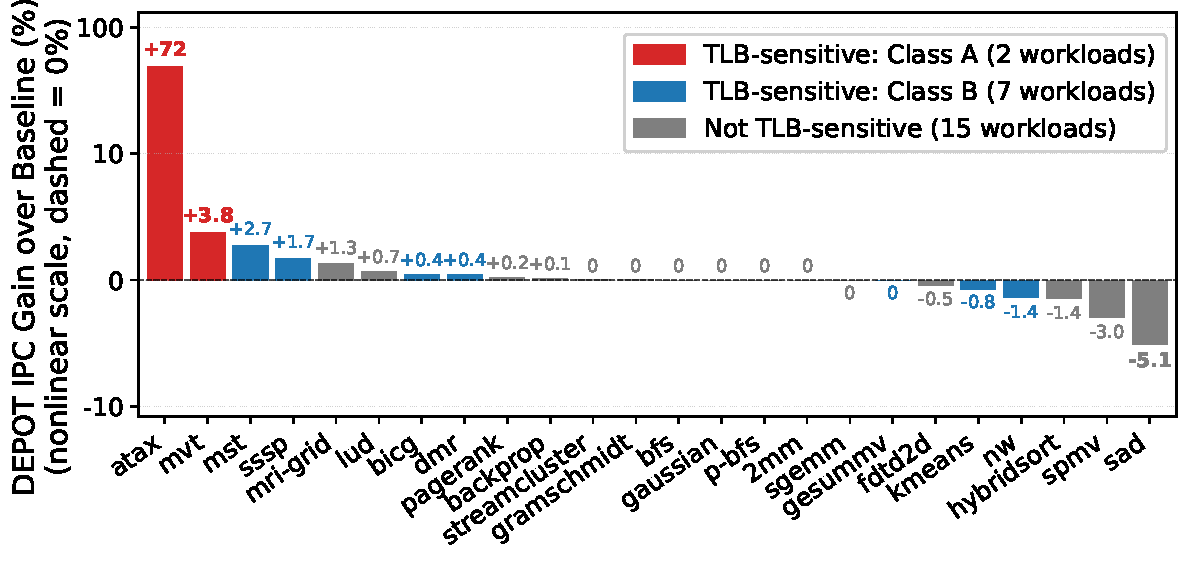
\includegraphics[width=\figwidth]{figs/fig09_o3_ipc_gains.pdf}
  \caption{IPC improvement of DEPOT over 4\,KB baseline for all 24 workloads, sorted descending.}
  \label{fig:o3_gains_bar}
\end{figure}

Figure~\ref{fig:o3_gains_bar} shows IPC improvement of DEPOT for all 24 workloads.
The results divide cleanly along the class boundaries established in
Section~\ref{sec:characterization}.
Among the 15 not-TLB-sensitive workloads, IPC improvement is near zero throughout, with
occasional small negative values including \texttt{sad} at $-5.1\%$ and \texttt{spmv}
at $-2.9\%$.
These minor regressions arise because DEPOT occasionally fires on workloads with
moderate DE ratios, marking re-installed entries as protected even though TLB misses
are not on their critical path; with MPKI of 0.02 and 0.19 respectively,
\texttt{sad} and \texttt{spmv} incur negligible TLB stall time at baseline,
so the observed losses reflect second-order LRU displacement rather than
translation overhead.
The LRU fallback bounds worst-case degradation but activates only when all entries
in a set are simultaneously protected, so partial-protection sets can still make
suboptimal eviction choices, which accounts for the small residual regression.
% These minor regressions arise from interactions between the modified replacement policy
% and moderate-DE-ratio workloads where the Bloom filter marks entries that are not
% performance-critical, slightly shifting eviction pressure onto others.
% In all 15 cases the workloads operate at the normalized IPC of well above 1.0, so the absolute cycle
% impact is negligible, and the LRU fallback limits worst-case degradation by design.
Among the two Class~A workloads, \texttt{atax} improves from 0.354 to 0.610 IPC for
a gain of $+72\%$, reflecting near-complete elimination of dead-entry re-walk stalls
that previously dominated its execution time.
\texttt{mvt} improves from 0.574 to 0.596 IPC for a gain of $+3.8\%$.
The smaller gain on \texttt{mvt} reflects its peak MSHR merge depth of 15 versus
\texttt{atax}'s 17 and its higher baseline IPC, indicating that TLB stalls already
represent a smaller fraction of its execution time before DEPOT is applied.
Both workloads converge to similar post-DEPOT IPC values near 0.60, consistent with
reaching a shared performance ceiling determined by compute throughput and memory
bandwidth rather than translation overhead.
All seven Class~B workloads show near-zero DEPOT gain, ranging from $-1.4\%$ to
$+2.7\%$, within simulation noise. This result holds across PolyBench, Lonestar, and Rodinia workloads: when each warp generates distinct VPNs, protecting one re-installed entry is immediately offset by another capacity eviction, while the LRU fallback ensures zero overhead.
\begin{comment}
All seven Class~B workloads show near-zero DEPOT gain, ranging from $-1.4\%$ to
$+2.7\%$, all within simulation noise. The result holds uniformly across PolyBench dense linear algebra, Lonestar graph workloads, and Rodinia clustering benchmarks: whenever each warp instruction generates
distinct VPNs, protecting any individual re-installed entry is immediately offset by a
new capacity eviction elsewhere, and the LRU fallback ensures zero overhead.
\end{comment}

\begin{figure}[ht]
  \centering
  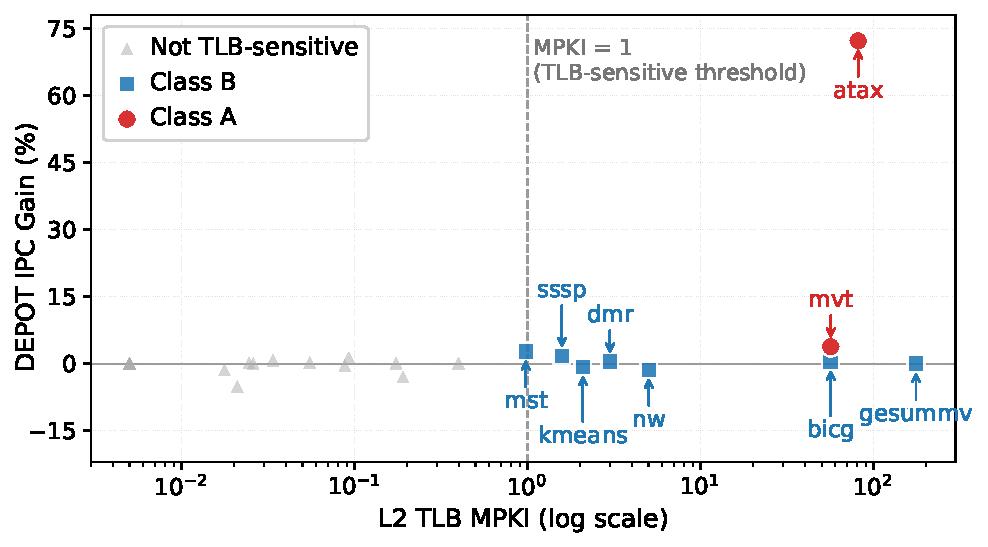
\includegraphics[width=\figwidth]{figs/fig11_o3gain_vs_mpki.pdf}
  \caption{IPC improvement of DEPOT vs.\ L2 TLB MPKI for all 24 workloads.}
  \label{fig:o3_scatter}
\end{figure}

Figure~\ref{fig:o3_scatter} plots IPC improvement of DEPOT against MPKI for all 24 workloads,
revealing a clean two-regime structure.
Workloads with MPKI below 1 cluster near zero gain regardless of their dead-entry ratio,
confirming that TLB miss rate is a necessary condition for sensitivity.
Within the high-MPKI group, workloads split by access structure: those with shared VPN
access show positive gains, while those with unique VPN access per warp show near-zero
gains.
The scatter plot makes visible what the aggregate bar chart in
Figure~\ref{fig:o3_gains_bar} obscures: MPKI identifies workloads for which TLB
behavior matters at all, while access structure determines whether eviction-history
protection can improve it.
To bound the overhead from false positives, we also evaluate a worst-case scenario with
a fully saturated Bloom filter, where every miss query returns a positive response
regardless of actual eviction history.
Under saturation, \texttt{atax} IPC remains at 0.610, identical to the normal DEPOT
result.
False positives cause DEPOT to protect entries that did not originate from dead-entry
re-walks, but the LRU fallback absorbs the resulting mismatch without measurable
performance impact, showing that the mechanism is tolerant of false positive pressure.

\begin{figure}[ht]
  \centering
  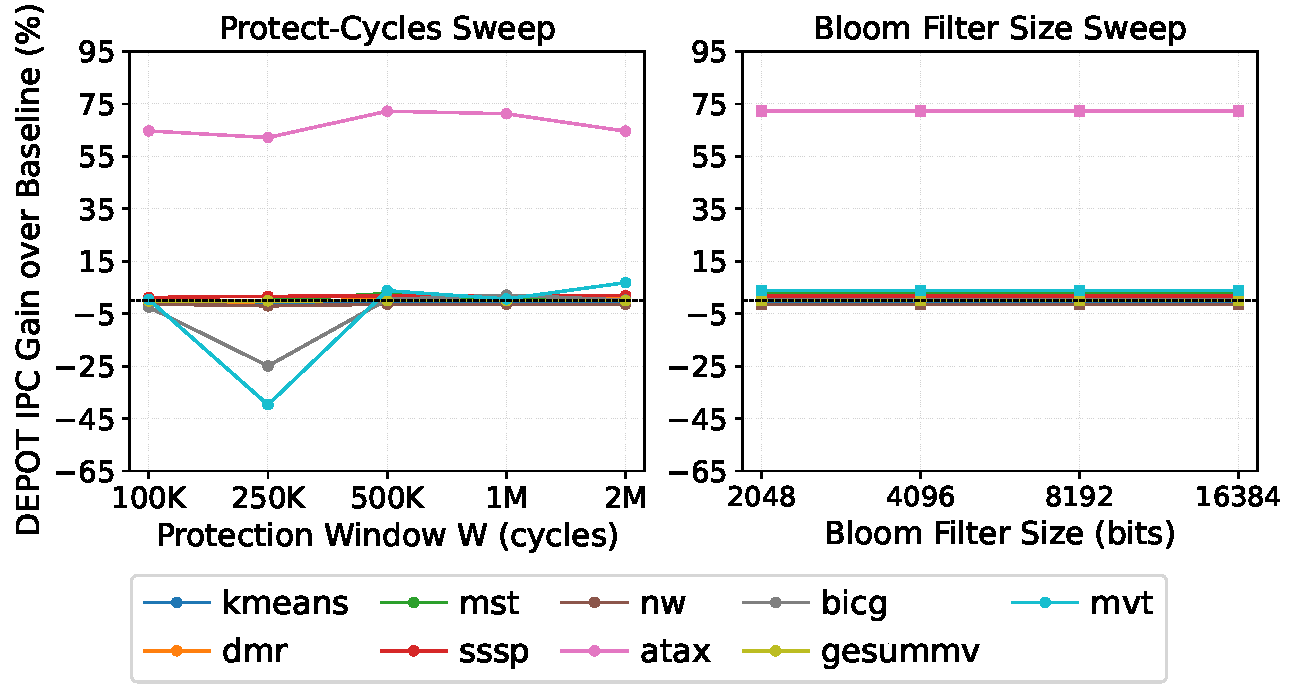
\includegraphics[width=\figwidth]{figs/fig13_param_sensitivity.pdf}
  \caption{DEPOT parameter sensitivity for 9 TLB-sensitive workloads: protection window $W$ (left) and Bloom filter size (right).}
  \label{fig:params}
\end{figure}

Figure~\ref{fig:params} shows DEPOT sensitivity to its two configurable parameters for 9 TLB-sensitive workloads. Both the protection-window sweep (100\,K to 2\,M) and Bloom-filter sweep (2048 to 16384 bits) remain nearly flat across the tested range. This indicates that TLB-sensitive workloads experience re-walk bursts within timescales covered by any reasonable protection window, while the eviction stream remains well below the saturation threshold of even the smallest Bloom filter. DEPOT is therefore robust to parameter choice, and the default configuration of a 500\,K-cycle protection window and an 8192-bit Bloom filter is effective across all evaluated workloads without tuning.

\begin{comment}
Figure~\ref{fig:params} shows the sensitivity of DEPOT to its two configurable
parameters for 9 TLB-sensitive workloads.
Both the protection window and the Bloom filter size sweeps are flat across the full
tested range, with the window varying from 100\,K to 2\,M cycles and the filter size
varying from 2048 to 16384 bits.
The insensitivity to window size reflects that TLB-sensitive workloads experience
re-walk events on timescales short enough that any reasonable protection duration covers
the relevant burst interval, so extending or shortening the window produces no
measurable change.
The insensitivity to filter size reflects that the eviction stream of TLB-sensitive
workloads is well below the saturation threshold of even the smallest tested
configuration, so adding more bits provides no additional discriminating power.
DEPOT is therefore robust to parameter choice, and the default configuration of a
500\,K-cycle protection window and an 8192-bit Bloom filter is safe across all
workloads tested without tuning.
\end{comment}

\subsection{Class~A/B Asymmetry}
\label{sec:disc_classes}
The performance asymmetry between Class A and Class B follows directly from the access-structure analysis in Section~\ref{sec:char_burstness} and explains both the large gains on \texttt{atax} and the near-zero results on the Class B workloads. In Class A workloads, a single dead-entry eviction is amplified through MSHR merging because many warps simultaneously reference the same virtual page. When DEPOT protects the re-installed entry, it eliminates both the initial re-walk and the merged re-walks that would otherwise stall many warps simultaneously. On SM86, page-walk latency is approximately 300–500 cycles, and releasing dozens of stalled warps with a single protection event can recover thousands of cycles, consistent with the observed +72\% IPC improvement.

In Class B workloads, by contrast, the TLB is continuously occupied by a working set that exceeds TLB reach, and each warp accesses distinct pages with little cross-warp sharing. Protecting one re-installed entry therefore only shifts the next eviction to another entry without reducing the overall eviction rate. Because MSHR merging is minimal, each page walk serves only one warp, so the benefit of protection is limited. When all entries are under protection pressure, DEPOT falls back to standard LRU replacement, ensuring negligible overhead in this regime.

\begin{comment}
The performance asymmetry between Class~A and Class~B follows directly from the access
structure analysis in Section~\ref{sec:char_burstness}, and understanding it explains
both the large gains on \texttt{atax} and the near-zero results on the Class~B workloads.
In Class~A workloads, a single dead-entry eviction is not an isolated event: because
many warps simultaneously reference the same virtual page, that eviction stalls all of
them at once through the MSHR merge mechanism.
When DEPOT protects the re-installed entry, it remains in the TLB through the entire
burst of warp accesses referencing that page, eliminating not just the first re-walk
but all of the merged re-walks in the burst simultaneously.
The result is that one protection decision avoids many stall cycles, and the compounding
effect is what produces the large observed IPC gain on \texttt{atax}.
The page-walk latency to DRAM on the SM86 microarchitecture is approximately 300 to
500 cycles, and when a burst of dozens of warps is unblocked by a single protection
event, the total recovered cycles per event can reach into the thousands, consistent
with the $+72\%$ IPC improvement observed.
In Class~B workloads, by contrast, the TLB entry pool is fully occupied by the working
set, and each warp accesses distinct pages with no cross-warp sharing.
Protecting one re-installed entry simply forces a different equally-soon-to-be-evicted
entry to absorb the next eviction instead, shifting which entry is displaced without
reducing how many evictions occur overall.
Because there is no MSHR merging, each page walk serves exactly one warp, and
protecting one entry saves at most one page-walk latency before a new capacity eviction
immediately regenerates a dead-entry miss at the same location.
The LRU fallback handles the case where all entries are simultaneously under protection
pressure by yielding to standard LRU, ensuring DEPOT imposes no overhead in this regime.
\end{comment}

\subsection{Composition with LatPC}
\label{sec:o3_latpc}

LatPC combines stride-based prefetching with entry compaction and represents the
state-of-the-art in GPU TLB optimization.
It trains a stride predictor for each TLB entry and issues prefetch requests before
demand misses occur, targeting cold and capacity-driven misses through access-pattern
prediction.
DEPOT and LatPC address fundamentally different sources of TLB misses: LatPC reduces
misses by predicting future accesses and filling the TLB ahead of demand, while DEPOT
reduces misses by preventing recently installed entries from being prematurely evicted
at the replacement boundary.
Because their mechanisms operate on different points in the TLB pipeline, one does not
subsume the other: on interference-driven workloads the two compose additively, while
on capacity-saturated workloads they can contend, as the results below show.

\begin{figure}[ht]
  \centering
  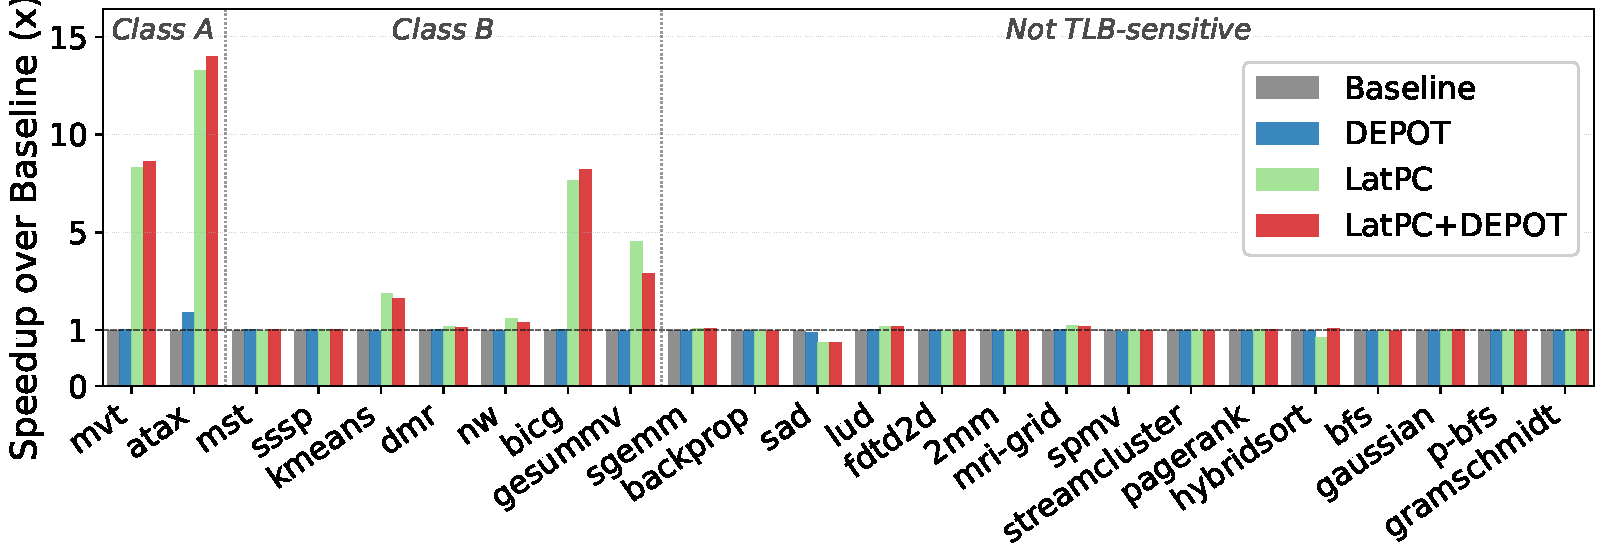
\includegraphics[width=\figwidth]{figs/fig10_ipc_comparison.pdf}
  \caption{IPC comparison across four configurations for all 24 workloads.}
  \label{fig:ipc}
\end{figure}

Figure~\ref{fig:ipc} shows the composition result across all configurations.
LatPC alone achieves large gains on TLB-sensitive workloads, with \texttt{atax}
improving by $+1227\%$ from 0.354 to 4.70\,IPC, \texttt{bicg} by $+667\%$ from 0.601
to 4.61\,IPC, and \texttt{mvt} by $+729\%$ from 0.574 to 4.76\,IPC.
These gains reflect LatPC's elimination of the dominant cold-miss bottleneck, which
accounts for the large majority of TLB stalls in these workloads.
LatPC+DEPOT outperforms LatPC alone on the Class~A workloads, with \texttt{atax}
improving further from 4.70 to 4.95\,IPC ($+5.4\%$) and \texttt{mvt} from 4.76 to
4.95\,IPC ($+4.0\%$).
Across the Class~B workloads, LatPC+DEPOT shows mixed results: \texttt{bicg}
($+6.9\%$), \texttt{mst} ($+2.5\%$), and \texttt{sssp} ($+2.1\%$) gain modestly,
\texttt{dmr} is negligible ($-0.9\%$), while \texttt{kmeans} ($-8.3\%$),
\texttt{nw} ($-10.0\%$), and \texttt{gesummv} ($-28.5\%$) regress.
These regressions arise because DEPOT's eviction-protection policy conflicts with
LatPC's prefetch-driven replacement in capacity-saturated workloads: LatPC must
freely evict entries to install ahead-of-demand translations, and DEPOT's protected
entries block those slots, delaying prefetch fills and causing net IPC loss.

The additive improvement on Class~A workloads arises because LatPC does not eliminate all
dead-entry re-walks even when its prefetcher is operating correctly.
The key reason is the asymmetry between what the prefetcher targets and what eviction
produces.
LatPC observes that a warp accesses VPN $A$, then predicts and prefetches the next
VPN in the stride sequence.
While the prefetch is in flight, VPN $A$ itself may be displaced from the TLB by LRU
replacement, because the prefetch installs a new entry and the LRU policy does not
know that $A$ will be accessed again at the next stride period.
When that next access to $A$ arrives it finds the entry gone, a dead-entry miss that
LatPC's forward-looking predictor cannot catch; DEPOT observes the eviction of $A$
at the replacement boundary and protects the re-installed entry, covering exactly
this residual class.
Where the combination is beneficial---the Class~A workloads and \texttt{bicg}---the
2 to 7\% additional IPC improvement reflects how frequently this interaction between
prefetch-driven installation and LRU displacement produces residual dead-entry events.
The marginal hardware cost of adding DEPOT to a LatPC-equipped TLB is a 1\,KB Bloom
filter, negligible relative to LatPC's per-entry stride prediction tables, making the
combination an efficient pairing for workloads that benefit from both.

\section{Discussion and Limitations}
\label{sec:discussion}

The 2\,MB page results in Section~\ref{sec:char_2mb} raise a natural question about whether
DEPOT is necessary if larger pages already resolve TLB pressure.
The two mechanisms address different root causes and are not interchangeable.
Larger pages expand TLB reach and directly relieve capacity eviction in Class~B workloads,
but they do not eliminate interference-driven eviction in Class~A workloads, nor are they
always available: GPU workloads frequently use custom memory pools or third-party libraries
that do not guarantee 2\,MB alignment, and virtualized environments may not expose huge page
support to guest workloads at all.
DEPOT operates entirely within the TLB microarchitecture and is transparent to the OS,
driver, and application, making it applicable in settings where large pages are unavailable
or impractical.

DEPOT targets interference-driven dead-entry misses and provides no benefit for workloads
whose TLB pressure arises from working-set overflow beyond the TLB reach.
The Class~B workloads in this study fall squarely into this regime, and the near-zero DEPOT
gains on those workloads confirm that eviction-history protection does not substitute for
additional TLB capacity or larger page mappings.
Practitioners diagnosing TLB performance issues should therefore use the two-class
characterization framework to identify the dominant root cause before selecting an
intervention, as applying DEPOT to a capacity-driven workload not only fails to improve performance
but can actively regress it when a prefetcher such as LatPC is also present,
by blocking the replacement slots that prefetch fills require.
% as applying DEPOT to a capacity-driven workload adds hardware overhead
% without providing a compensating benefit.

Composition with an aggressive prefetcher is a further limitation.
DEPOT applied alone never regresses, but composing it with LatPC is not universally
additive: on three capacity-driven Class~B workloads---\texttt{kmeans}, \texttt{nw},
and \texttt{gesummv}---LatPC+DEPOT regresses relative to LatPC alone (by $8.3\%$,
$10.0\%$, and $28.5\%$ respectively), as DEPOT's protection window and LatPC's
prefetch installs contend for L2 TLB capacity.
This is consistent with the taxonomy rather than a counterexample to it: DEPOT is an
interference-driven (Class~A) optimization, and these regressions occur only when it
is misapplied to capacity-driven workloads atop a prefetcher.
A capacity-aware coupling of the two mechanisms---for instance, suspending protection
while the prefetcher is actively installing---is a worthwhile direction for future work.

The evaluation in this paper is conducted on the SM86 Ampere microarchitecture using a
validated simulation model.
The qualitative behavior of dead-entry misses, including MSHR-merge amplification and the
distinction between interference-driven and capacity-driven eviction, is expected to
generalize across GPU microarchitectures that share the same L1 and L2 TLB organization.
However, the specific quantitative thresholds used to classify workloads and the absolute
IPC improvement reported here are calibrated to SM86 parameters such as the 1024-entry L2 TLB
capacity and 16 hardware page-table walkers, and may differ on architectures with
substantially different TLB configurations.
